\chapter{Magnification coefficients}
This chapter studies if it is indeed necessary to recalculate the magnification coefficients for each iteration.\\

\section{Overview magnification coefficients}
The magnification coefficients transform the values obtained in the fit (namely $\Theta^z_{p,s} $ and $\Theta^y_{p,s} $) to the 2D histograms of the Cherenkov angle resolution vs azimuthal angle $\Phi$ to the actual mirror tilts.\\
\begin{figure}[!ht]
	\vspace*{-0.cm}
	\begin{center}
		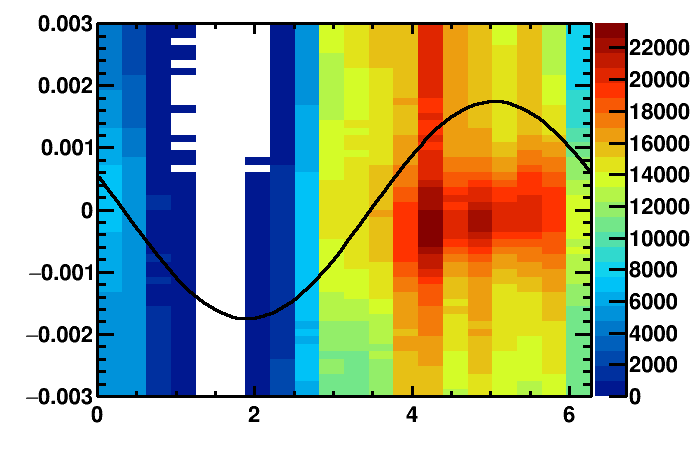
\includegraphics[width=0.7\textwidth]{dThetavphiRec4731.png}
		\vspace*{-1.cm}
	\end{center}
	\caption{\textit{Example of a fit to the 2D histograms of the Cherenkov angle resolution $\delta \theta_{p,s}$ vs azimuthal angle $\Phi$. Fit function: $\delta \theta_{p,s}(\Phi) = \Theta^z_{p,s} \cos\Phi + \Theta^y_{p,s} \sin\Phi$ .} }
	\label{fig:fitfunc}
\end{figure}
The magnification coefficients $A^y_{p,s}$, $A^z_{p,s}$, $B^y_{p,s}$ and $B^z_{p,s}$ relate the fit-values $\Theta^z_{p,s} $ and $\Theta^y_{p,s} $ to the actual mirror tilts $\alpha^y_p$, $\alpha^z_p$, $\beta^y_s$ and $\beta^z_s$ using the following expression\\
\begin{figure}[!ht]
	\vspace*{-0.cm}
	\begin{center}
		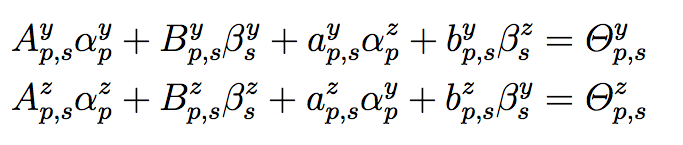
\includegraphics[width=0.5\textwidth]{magformular.png}
		\vspace*{-1.cm}
	\end{center}
\end{figure}
In this notation the index $_p$ stands for \textit{primary mirror}, $_s$ for \textit{secondary mirror}, $_{p,s}$ for a certain pair of primary and secondary mirror. The superscript $^y$ denotes a rotation around the $y$-axis and $^z$ around the $z$-axis.\\
\\
From the rich alignment paper (LHCb-INT-2013-007):\\
\textit{For each mirror combination the magnification factors are evaluated by introducing 8 independent calibrational rotations (positive or negative rotations about the $y$− or $z$−axes for the primary or secondary mirrors) and by measuring the resulting total tilts. In particular, $\pm 0.3\, mrad$ rotations are used. That choice is motivated by the fact that typically, Cherenkov angle resolution, the half-width of the $\theta$ distribution, for RICH2 is around $0.7\, mrad$. The final value of each factor is arithmetical mean of the two corresponding values obtained with the calibrating rotations in opposite directions.}
\\
\\
In the following section I have documented the evolution of the magnification coefficients over the course of an entire alignment.\\

\section{RICH1}
\subsection{Alignment from 17/06/2015 (not converged, offline)}
The plots below were made from the results of the first alignment performed on the 2015 data - starting from the last 2012 alignment. This alignment never converged.\\
Figure \ref{fig:rich12d_1} shows the distribution of the four different magnification coefficients of all mirror-pairs over the course of the entire alignment (10 iterations). The top plots just show the distribution of the magnification coefficients related to the primary mirrors while the bottom plots show the histograms of the mirror-tilts against their magnification coefficients (the primary mirrors of RICH1 are not tilted in the alignment procedure).\\

\begin{figure}[!ht]
	\vspace*{-0.cm}
	\begin{center}
		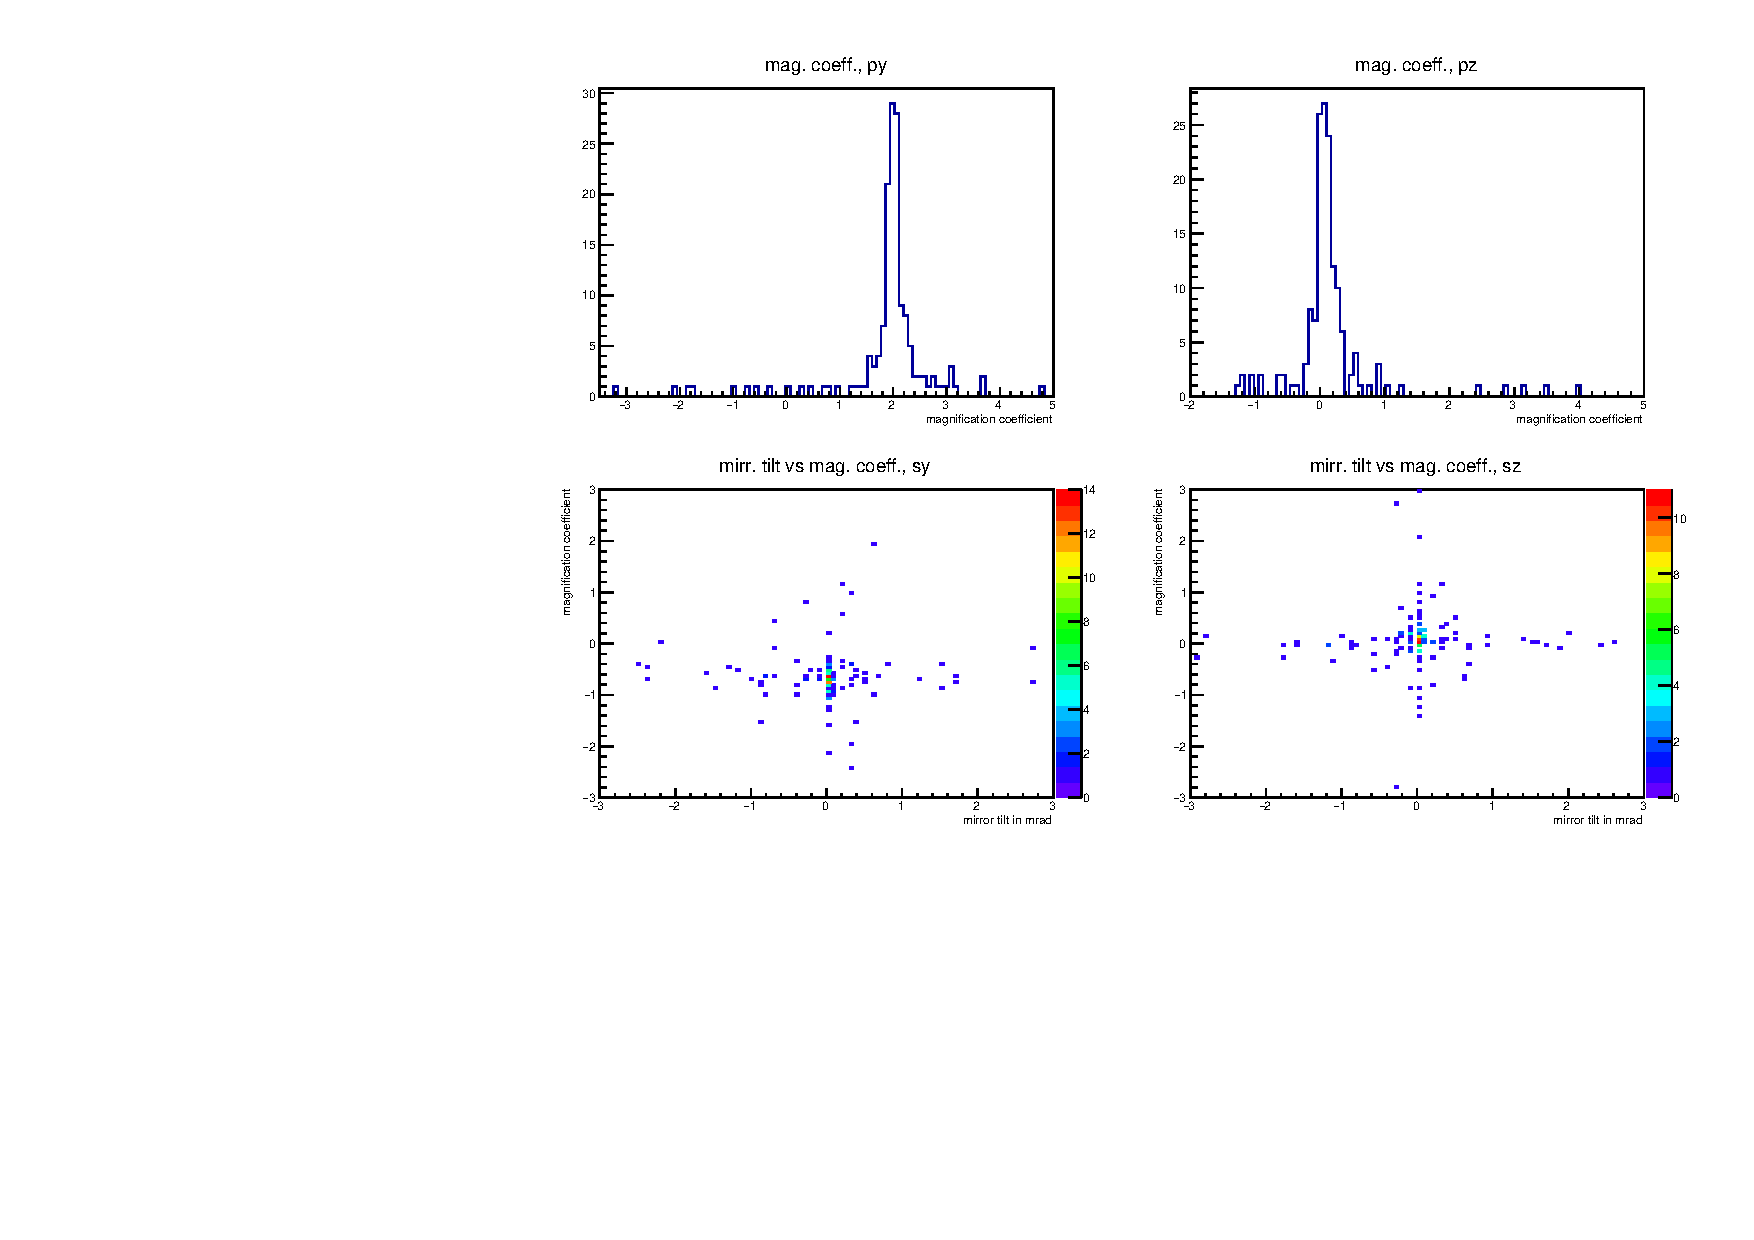
\includegraphics[width=1.\textwidth]{2dplot_rich1_1.pdf}
		\vspace*{-1.5cm}
	\end{center}
	\caption{\textit{Top plots: distribution of the magnification coefficients related to the primary mirrors; bottom plots: mirror-tilts against their magnification coefficients.}}
	\label{fig:rich12d_1}
\end{figure}
\\
Figures \ref{fig:rich1mag1_1} and \ref{fig:rich1mag2_1} show the development of the magnification coefficients for each mirror pair over the iterations of the alignment.\\
\begin{figure}[!ht]
	\vspace*{-0.cm}
	\begin{center}
		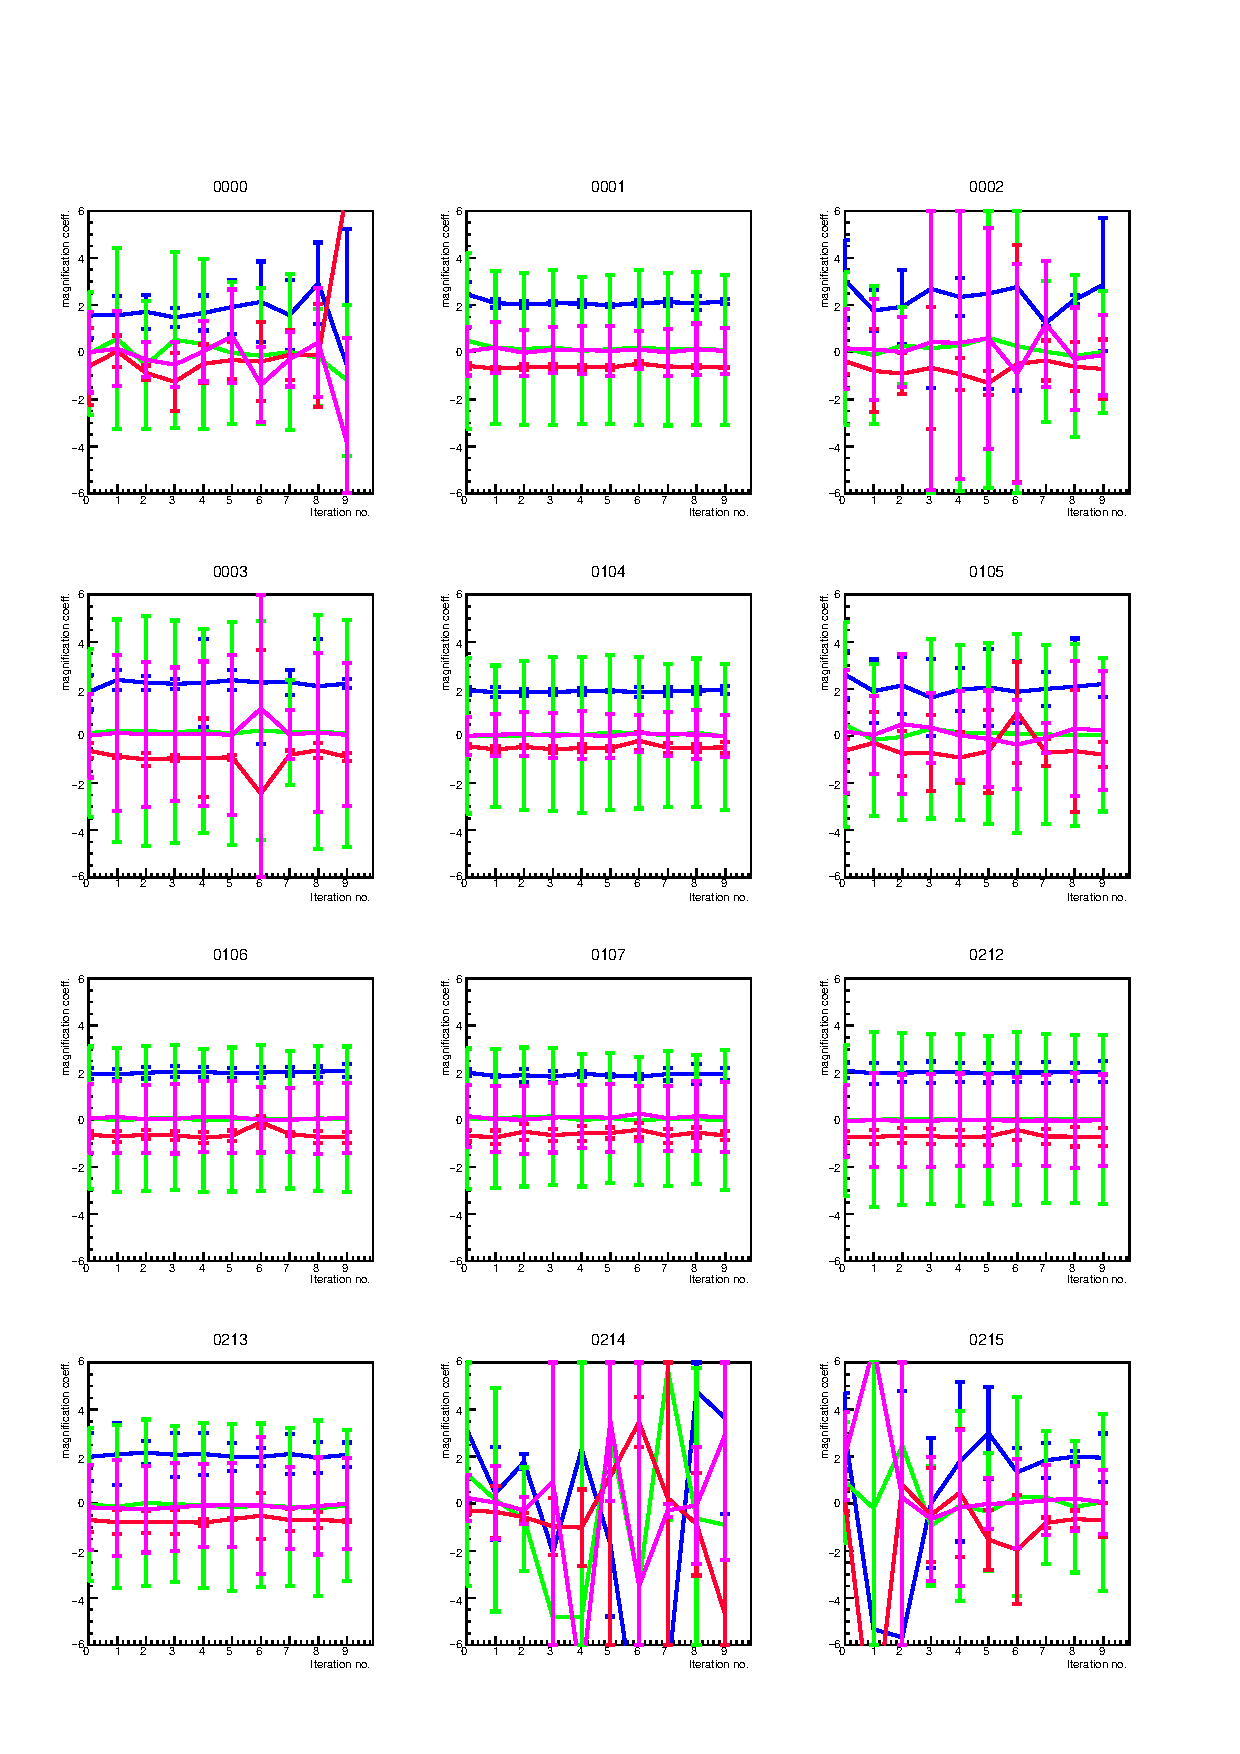
\includegraphics[width=1.\textwidth]{rich1_mag1_1.pdf}
		\vspace*{-1.5cm}
	\end{center}
	\caption{\textit{Development of the magnification coefficients for each mirror pair over the iterations of the alignment. Blue: rotation of primary mirror around y-axis, green: rotation of primary mirror around z-axis; red: rotation of secondary mirror around y-axis; magenta: rotation of secondary mirror around z-axis.}}
	\label{fig:rich1mag1_1}
\end{figure}

\begin{figure}[!ht]
	\vspace*{-0.cm}
	\begin{center}
		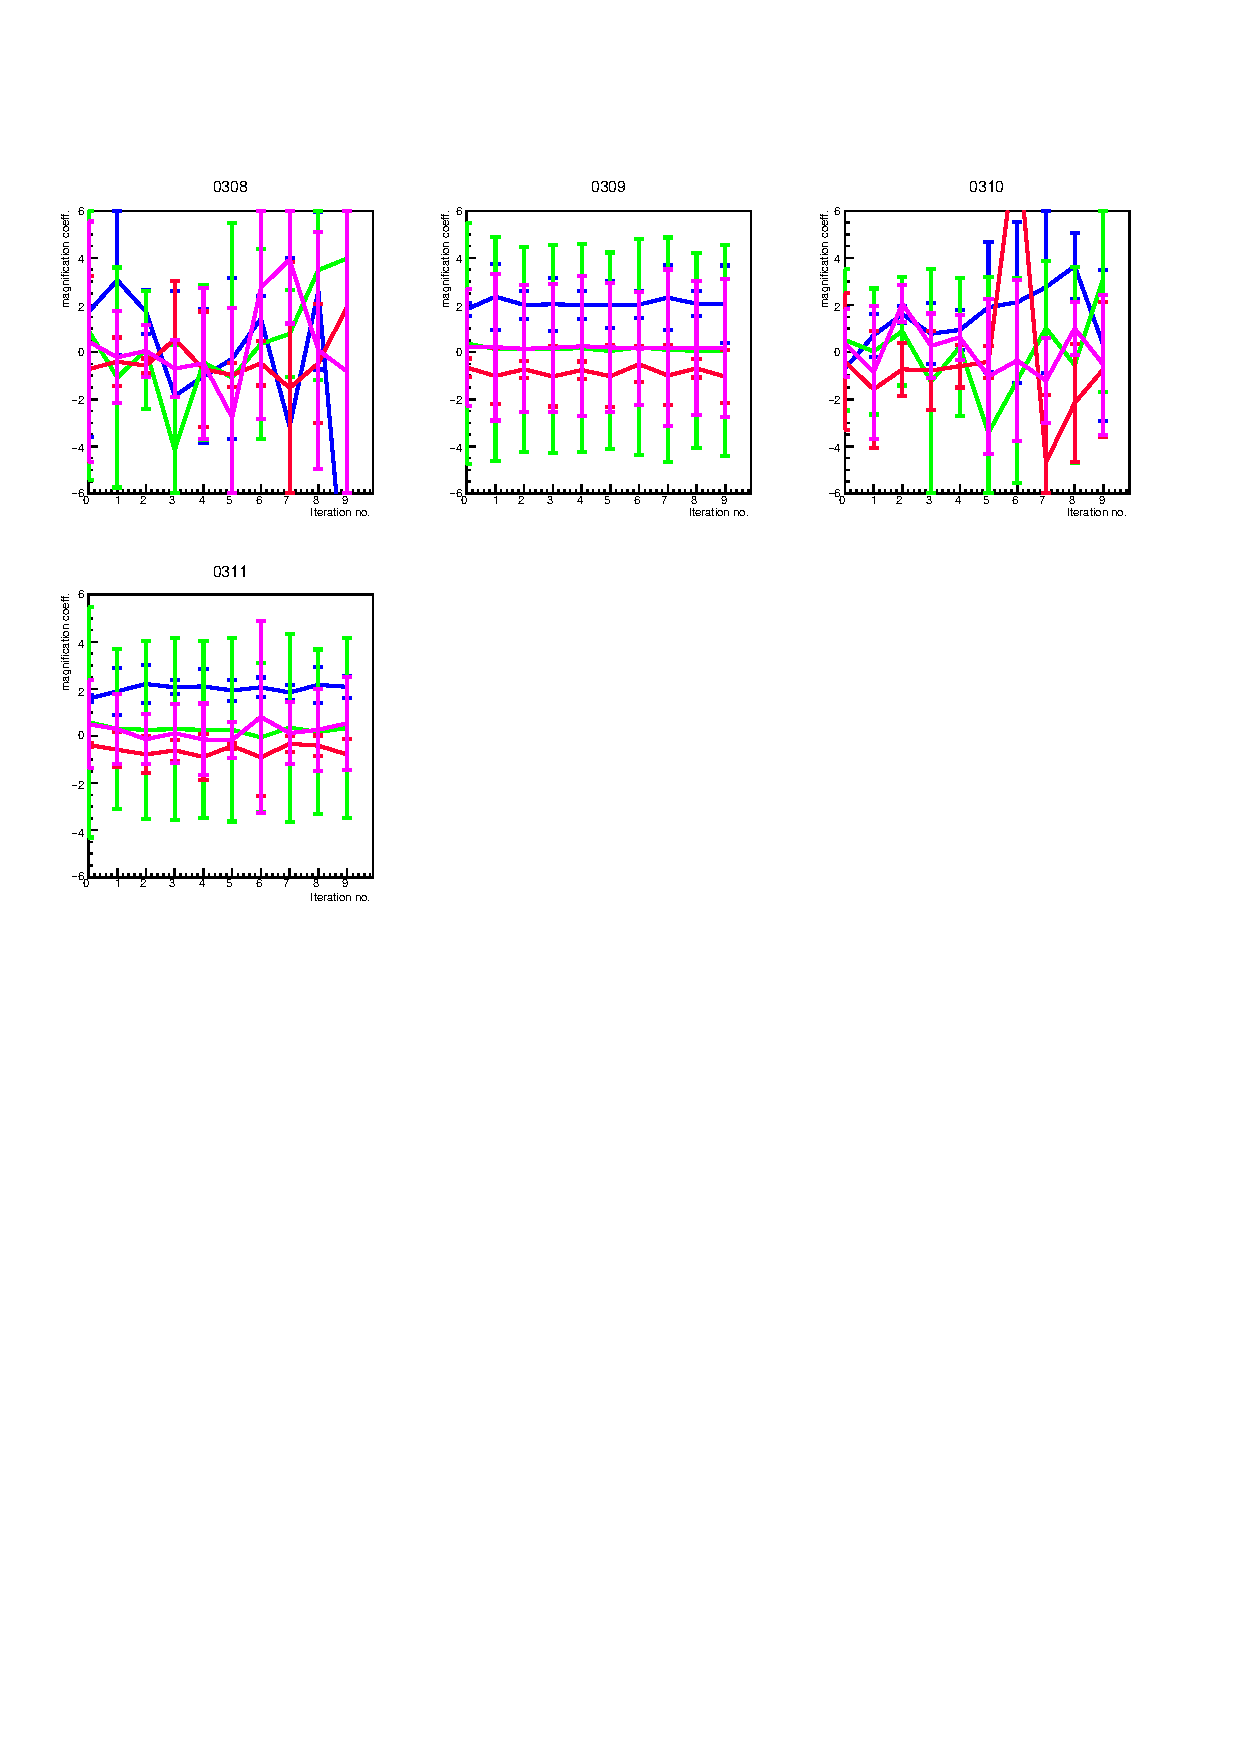
\includegraphics[width=1.\textwidth]{rich1_mag2_1.pdf}
		\vspace*{-1.5cm}
	\end{center}
	\caption{\textit{Development of the magnification coefficients for each mirror pair over the iterations of the alignment. Blue: rotation of primary mirror around y-axis, green: rotation of primary mirror around z-axis; red: rotation of secondary mirror around y-axis; magenta: rotation of secondary mirror around z-axis.}}
	\label{fig:rich12d_1}
\end{figure}

\clearpage
\subsection{Alignment from 11/07/2015 (fully converged, online)}
The plots below were made from the output of the fully converged alignment from 11/07/2015 which is at present time the latest RICH1 alignment. This alignment converged after 3 iterations.\\
Figure \ref{fig:rich12d_2} shows the distribution of the four different magnification coefficients of all mirror-pairs over the course of the entire alignment. The top plots just show the distribution of the magnification coefficients related to the primary mirrors while the bottom plots show the histograms of the mirror-tilts against their magnification coefficients (the primary mirrors of RICH1 are not tilted in the alignment procedure).\\
\\ 
\begin{figure}[!ht]
	\vspace*{-0.cm}
	\begin{center}
		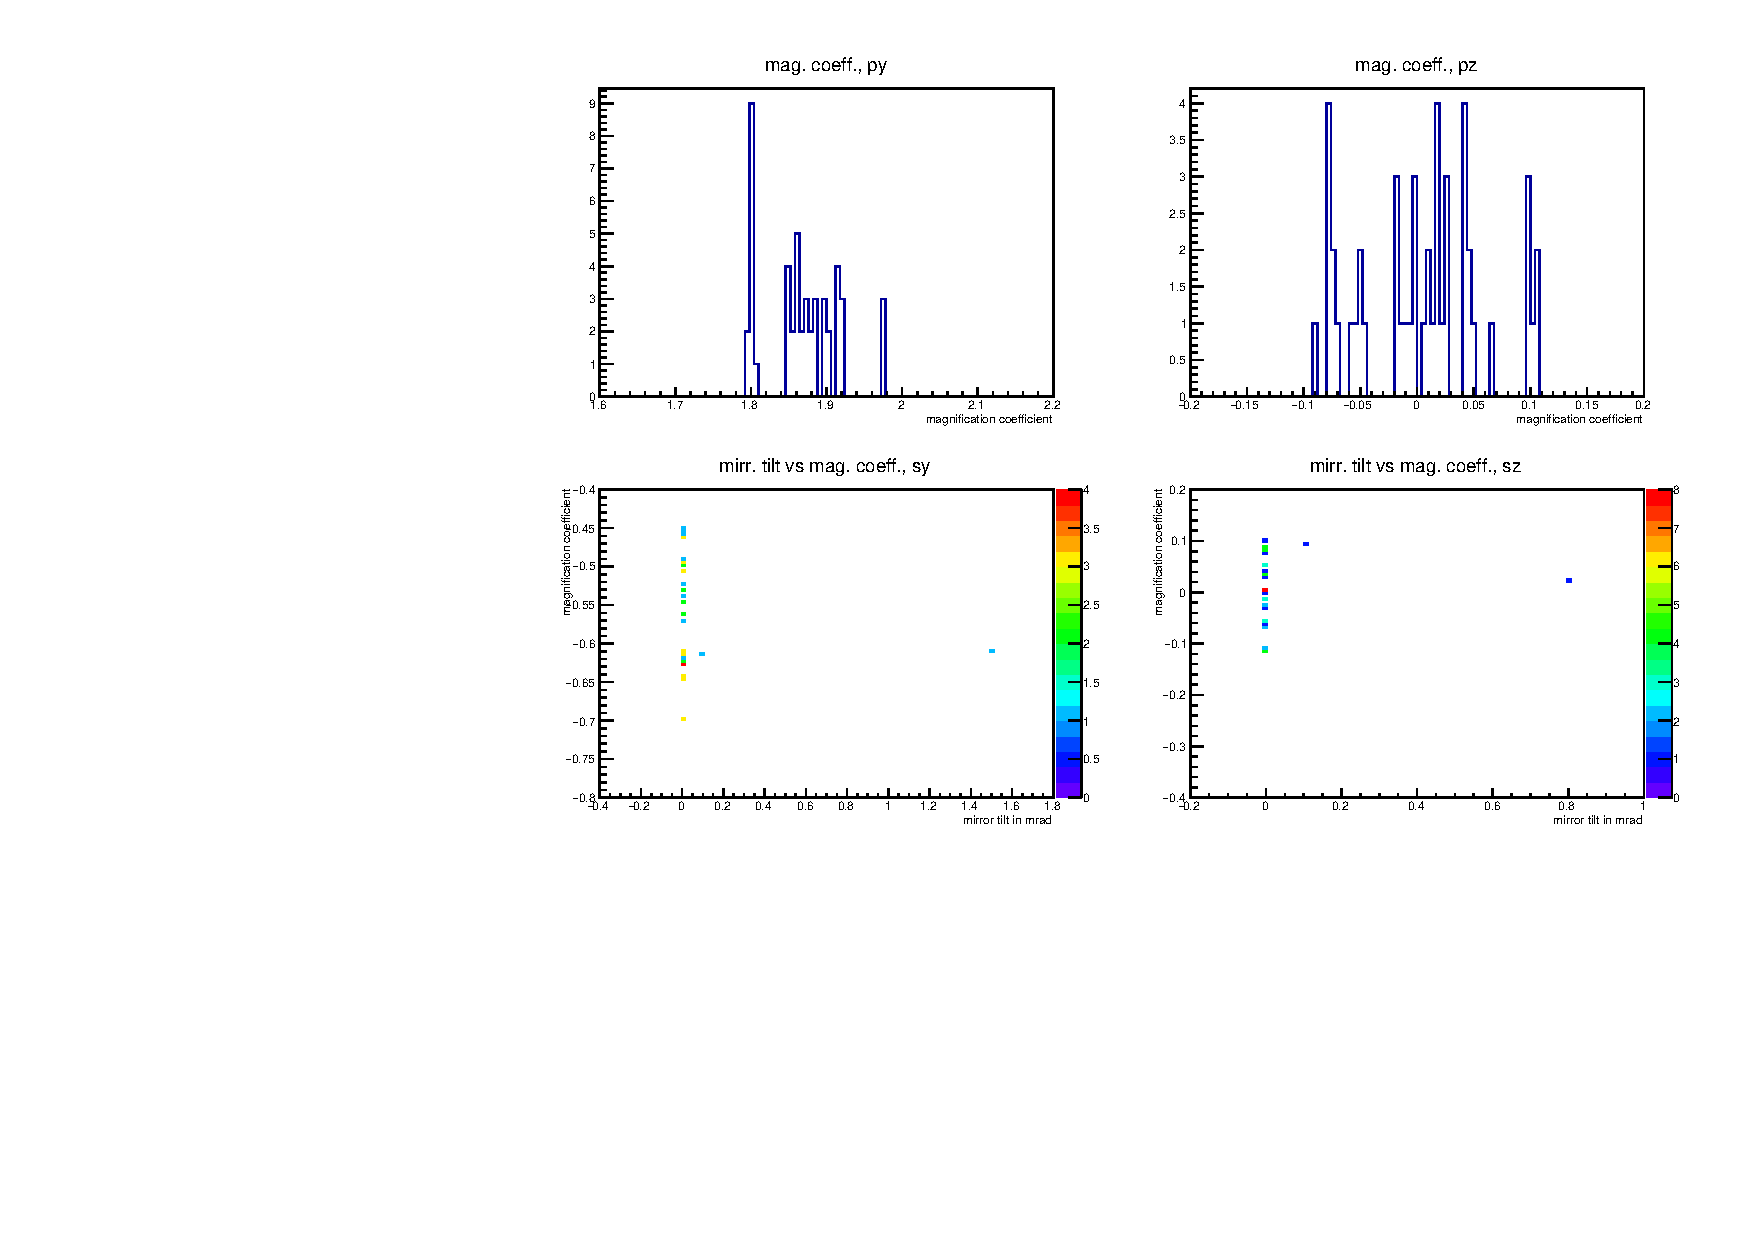
\includegraphics[width=1.\textwidth]{2dplot_rich1_2.pdf}
		\vspace*{-1.5cm}
	\end{center}
	\caption{\textit{Top plots: distribution of the magnification coefficients related to the primary mirrors; bottom plots: mirror-tilts against their magnification coefficients.}}
	\label{fig:rich12d_2}
\end{figure}
\\
Figures \ref{fig:rich1mag1_2} and \ref{fig:rich1mag2_2} show the development of the magnification coefficients for each mirror pair over the iterations of the alignment.\\
\begin{figure}[!ht]
	\vspace*{-0.cm}
	\begin{center}
		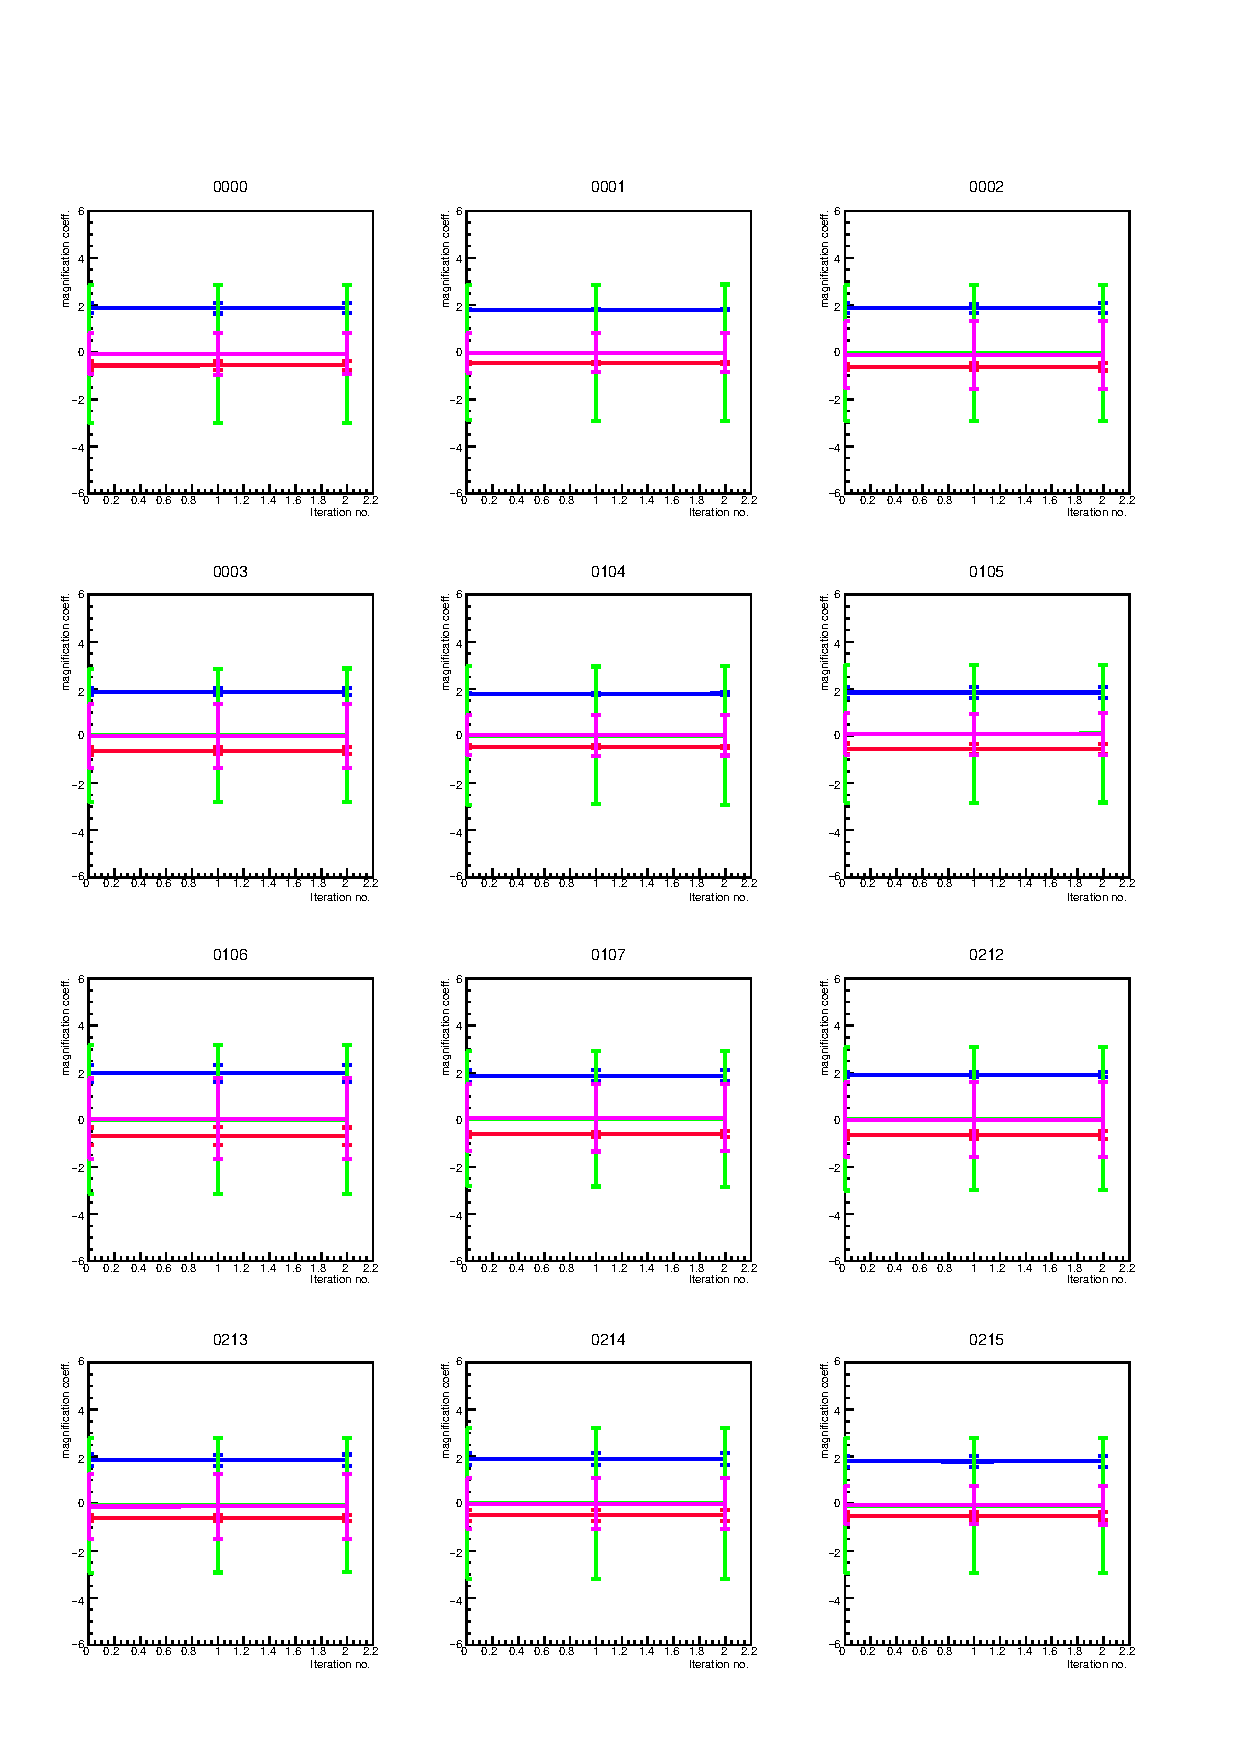
\includegraphics[width=1.\textwidth]{rich1_mag1_2.pdf}
		\vspace*{-1.5cm}
	\end{center}
	\caption{\textit{Development of the magnification coefficients for each mirror pair over the iterations of the alignment. Blue: rotation of primary mirror around y-axis, green: rotation of primary mirror around z-axis; red: rotation of secondary mirror around y-axis; magenta: rotation of secondary mirror around z-axis.}}
	\label{fig:rich1mag1_2}
\end{figure}

\begin{figure}[!ht]
	\vspace*{-0.cm}
	\begin{center}
		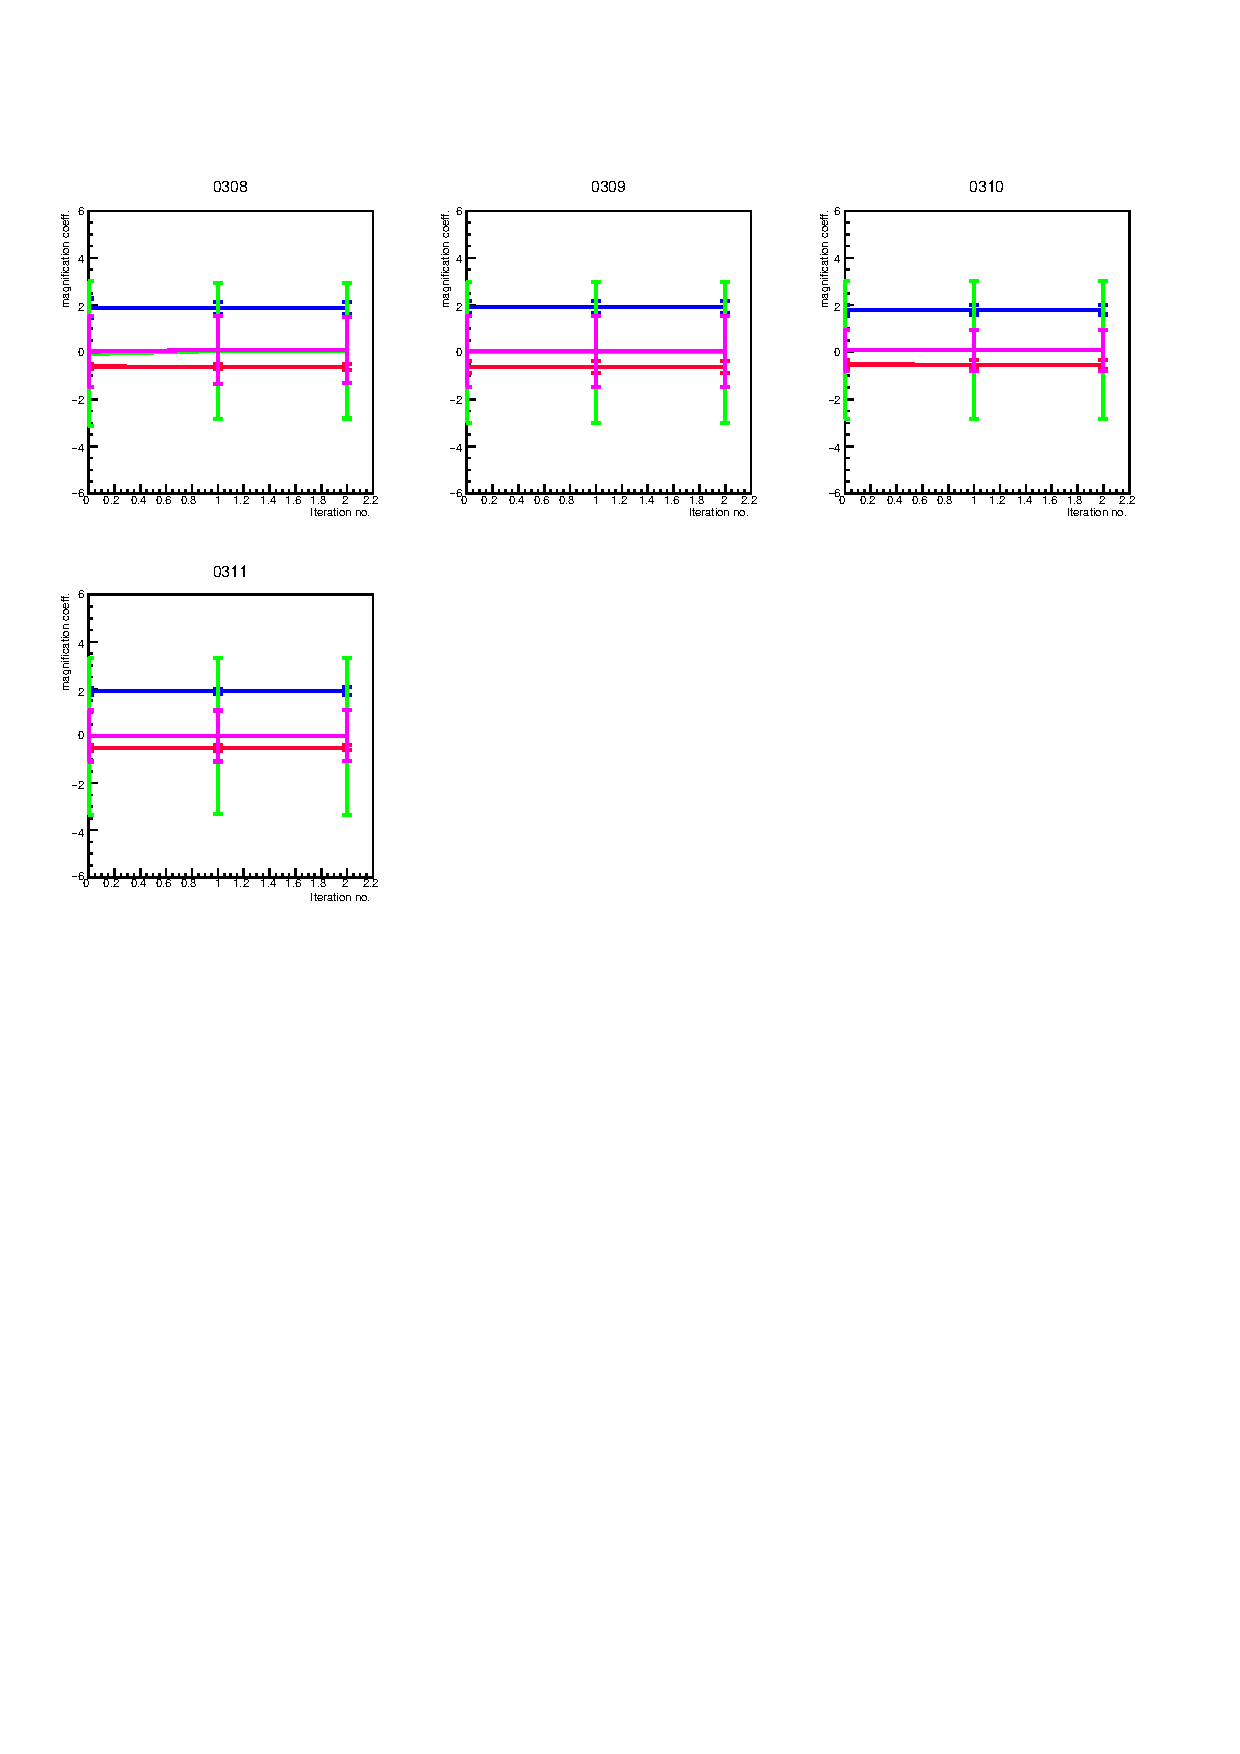
\includegraphics[width=1.\textwidth]{rich1_mag2_2.pdf}
		\vspace*{-1.5cm}
	\end{center}
	\caption{\textit{Development of the magnification coefficients for each mirror pair over the iterations of the alignment. Blue: rotation of primary mirror around y-axis, green: rotation of primary mirror around z-axis; red: rotation of secondary mirror around y-axis; magenta: rotation of secondary mirror around z-axis.}}
	\label{fig:rich1mag2_2}
\end{figure}
\clearpage


\section{RICH2}
\subsection{Alignment from 17/06/2015 (fully converged, offline)}
The plots below were made from the results of the first alignment performed on the 2015 data - starting from the last 2012 alignment. This alignment converged after 4 iterations.\\\\
Figure \ref{fig:rich22d_1} shows the distribution of the four different magnification coefficients of all mirror-pairs over the course of the entire alignment.\\
\begin{figure}[!ht]
	\vspace*{-0.cm}
	\begin{center}
		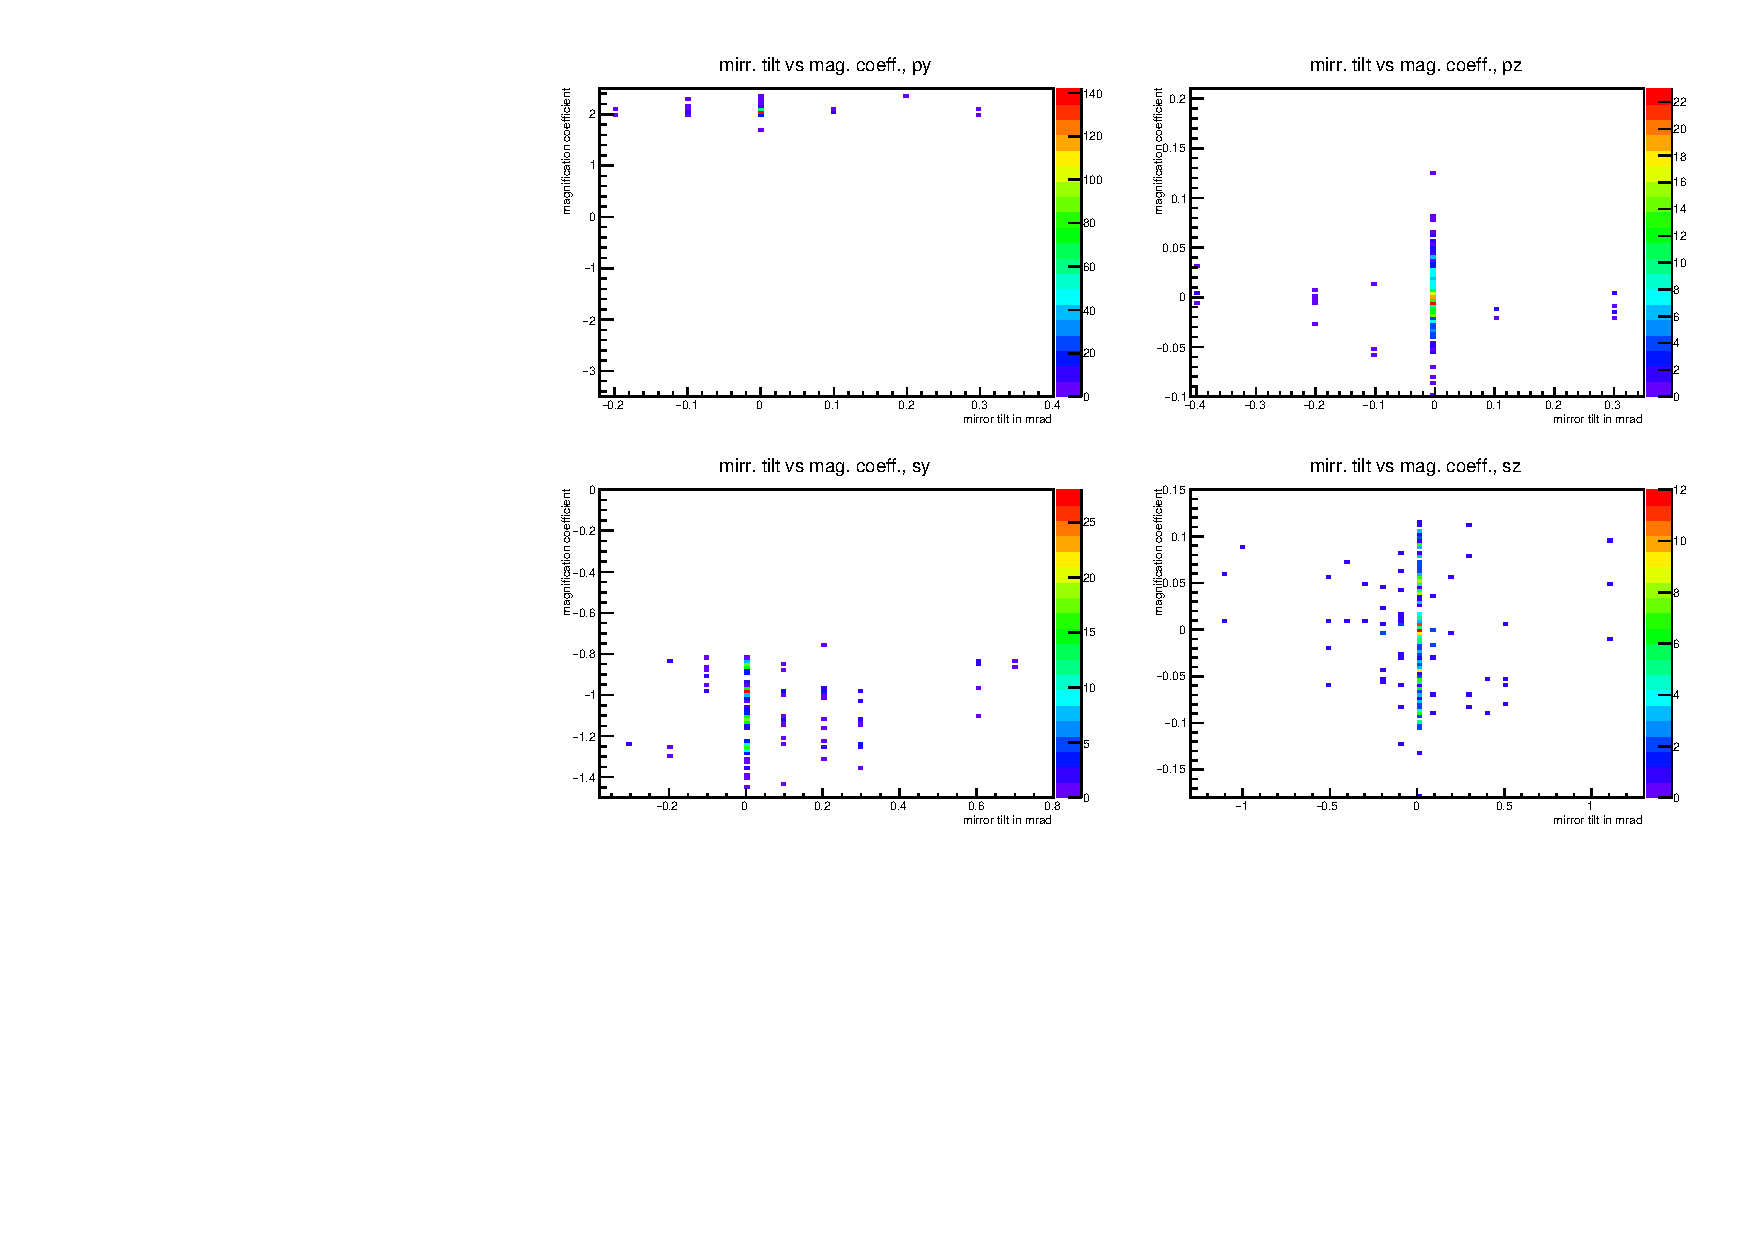
\includegraphics[width=1.\textwidth]{2dplot_rich2_1.pdf}
		\vspace*{-1.5cm}
	\end{center}
	\caption{\textit{Mirror-tilts against their magnification coefficients.}}
	\label{fig:rich22d_2}
\end{figure}
\\
Figures \ref{fig:rich2mag1_1} to \ref{fig:rich2mag2_8} show the development of the magnification coefficients for each mirror pair over the iterations of the alignment.\\
\begin{figure}[!ht]
	\vspace*{-0.cm}
	\begin{center}
		\includegraphics[width=1.\textwidth]{rich2_mag1_1.pdf}
		\vspace*{-1.5cm}
	\end{center}
	\caption{\textit{Development of the magnification coefficients for each mirror pair over the iterations of the alignment. Blue: rotation of primary mirror around y-axis, green: rotation of primary mirror around z-axis; red: rotation of secondary mirror around y-axis; magenta: rotation of secondary mirror around z-axis.}}
	\label{fig:rich2mag1_1}
\end{figure}

\begin{figure}[!ht]
	\vspace*{-0.cm}
	\begin{center}
		\includegraphics[width=1.\textwidth]{rich2_mag2_1.pdf}
		\vspace*{-1.5cm}
	\end{center}
	\caption{\textit{Development of the magnification coefficients for each mirror pair over the iterations of the alignment. Blue: rotation of primary mirror around y-axis, green: rotation of primary mirror around z-axis; red: rotation of secondary mirror around y-axis; magenta: rotation of secondary mirror around z-axis.}}
	\label{fig:rich2mag2_1}
\end{figure}
\begin{figure}[!ht]
	\vspace*{-0.cm}
	\begin{center}
		\includegraphics[width=1.\textwidth]{rich2_mag3_1.pdf}
		\vspace*{-1.5cm}
	\end{center}
	\caption{\textit{Development of the magnification coefficients for each mirror pair over the iterations of the alignment. Blue: rotation of primary mirror around y-axis, green: rotation of primary mirror around z-axis; red: rotation of secondary mirror around y-axis; magenta: rotation of secondary mirror around z-axis.}}
	\label{fig:rich2mag3_1}
\end{figure}
\begin{figure}[!ht]
	\vspace*{-0.cm}
	\begin{center}
		\includegraphics[width=1.\textwidth]{rich2_mag4_1.pdf}
		\vspace*{-1.5cm}
	\end{center}
	\caption{\textit{Development of the magnification coefficients for each mirror pair over the iterations of the alignment. Blue: rotation of primary mirror around y-axis, green: rotation of primary mirror around z-axis; red: rotation of secondary mirror around y-axis; magenta: rotation of secondary mirror around z-axis.}}
	\label{fig:rich2mag4_1}
\end{figure}
\begin{figure}[!ht]
	\vspace*{-0.cm}
	\begin{center}
		\includegraphics[width=1.\textwidth]{rich2_mag5_1.pdf}
		\vspace*{-1.5cm}
	\end{center}
	\caption{\textit{Development of the magnification coefficients for each mirror pair over the iterations of the alignment. Blue: rotation of primary mirror around y-axis, green: rotation of primary mirror around z-axis; red: rotation of secondary mirror around y-axis; magenta: rotation of secondary mirror around z-axis.}}
	\label{fig:rich2mag5_1}
\end{figure}
\begin{figure}[!ht]
	\vspace*{-0.cm}
	\begin{center}
		\includegraphics[width=1.\textwidth]{rich2_mag6_1.pdf}
		\vspace*{-1.5cm}
	\end{center}
	\caption{\textit{Development of the magnification coefficients for each mirror pair over the iterations of the alignment. Blue: rotation of primary mirror around y-axis, green: rotation of primary mirror around z-axis; red: rotation of secondary mirror around y-axis; magenta: rotation of secondary mirror around z-axis.}}
	\label{fig:rich2mag6_1}
\end{figure}
\begin{figure}[!ht]
	\vspace*{-0.cm}
	\begin{center}
		\includegraphics[width=1.\textwidth]{rich2_mag7_1.pdf}
		\vspace*{-1.5cm}
	\end{center}
	\caption{\textit{Development of the magnification coefficients for each mirror pair over the iterations of the alignment. Blue: rotation of primary mirror around y-axis, green: rotation of primary mirror around z-axis; red: rotation of secondary mirror around y-axis; magenta: rotation of secondary mirror around z-axis.}}
	\label{fig:rich2mag7_1}
\end{figure}
\begin{figure}[!ht]
	\vspace*{-0.cm}
	\begin{center}
		\includegraphics[width=1.\textwidth]{rich2_mag8_1.pdf}
		\vspace*{-1.5cm}
	\end{center}
	\caption{\textit{Development of the magnification coefficients for each mirror pair over the iterations of the alignment. Blue: rotation of primary mirror around y-axis, green: rotation of primary mirror around z-axis; red: rotation of secondary mirror around y-axis; magenta: rotation of secondary mirror around z-axis.}}
	\label{fig:rich2mag8_1}
\end{figure}



\clearpage




\subsection{Alignment from 19/07/2015 (fully converged, online)}
The plots below were made from the output of the fully converged alignment from 19/07/2015 which is at present time the latest RICH1 alignment. This alignment converged after 3 iterations.\\
Figure \ref{fig:rich22d_2} shows the distribution of the four different magnification coefficients of all mirror-pairs over the course of the entire alignment. \\
\begin{figure}[!ht]
	\vspace*{-0.cm}
	\begin{center}
		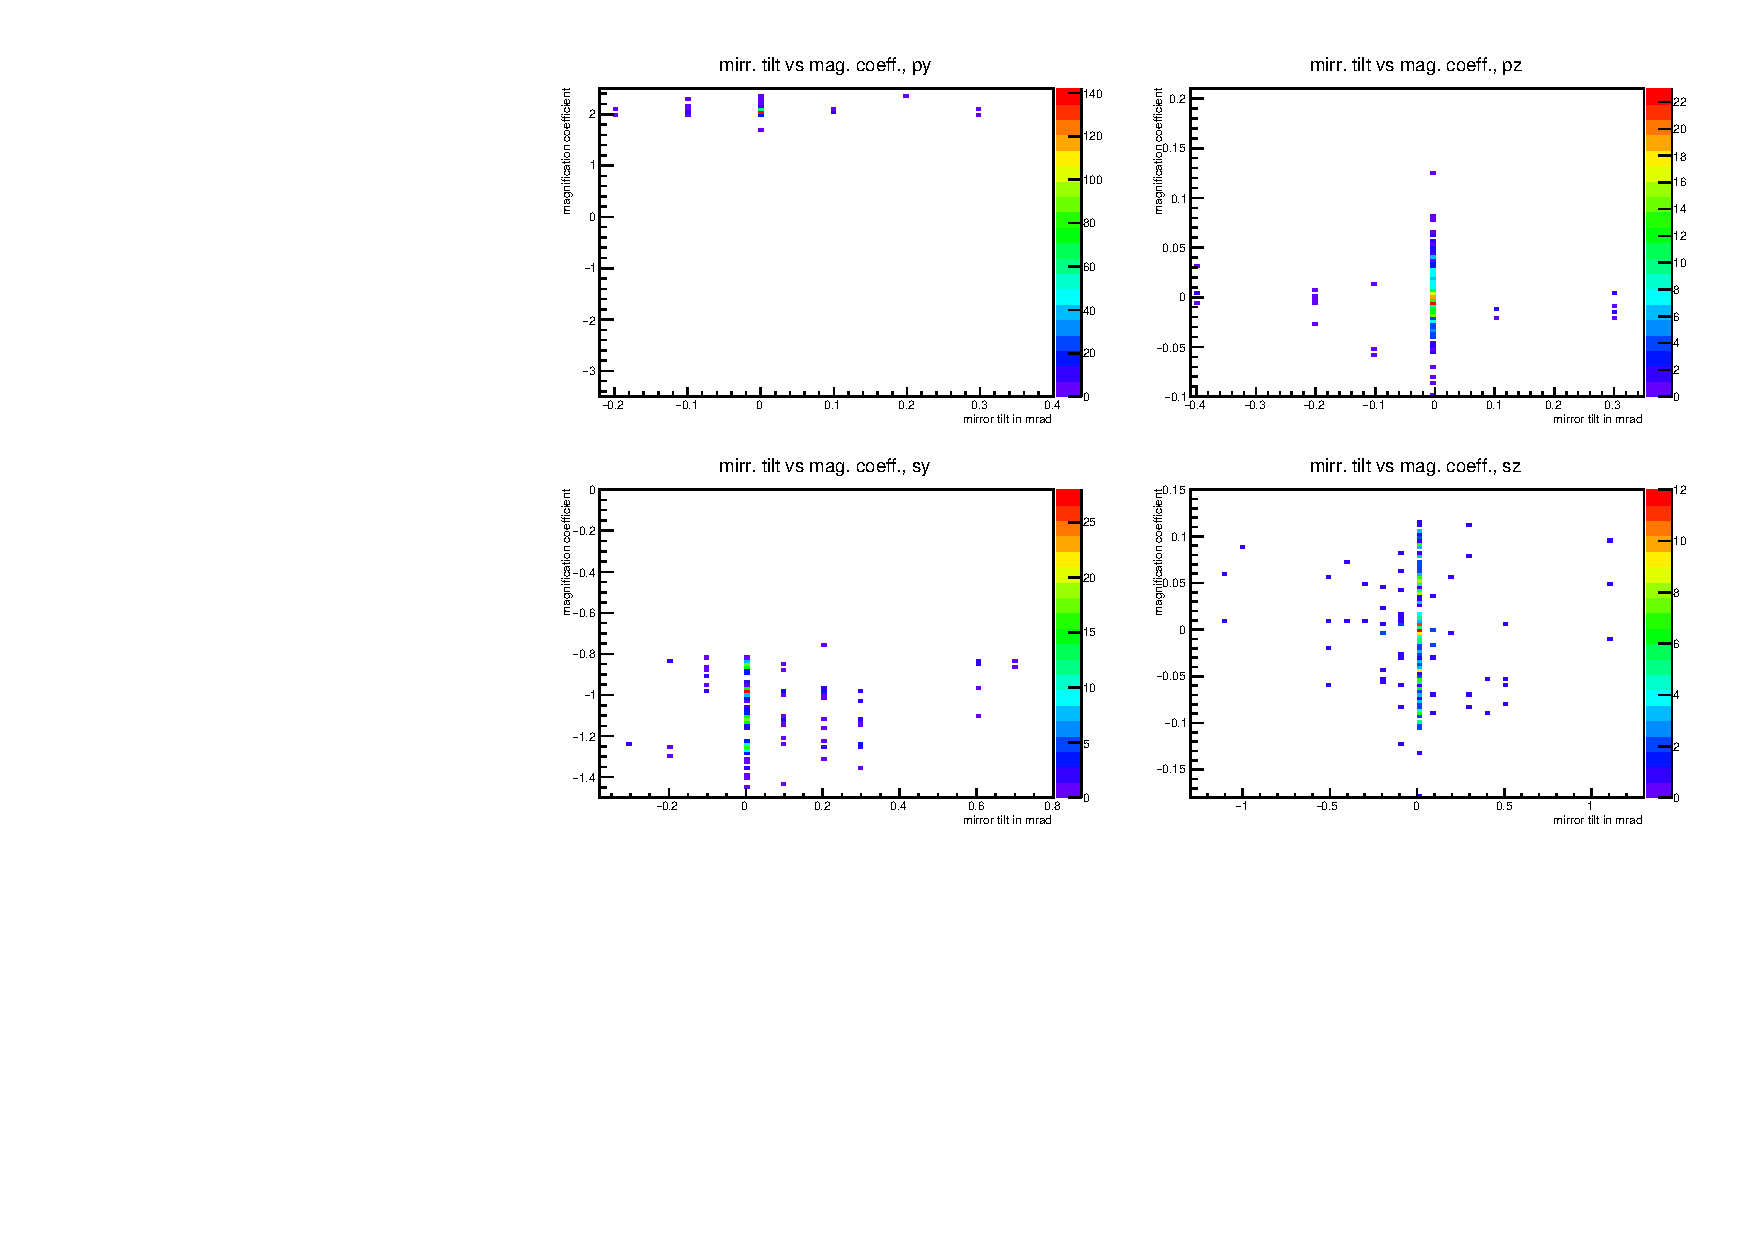
\includegraphics[width=1.\textwidth]{2dplot_rich2_1.pdf}
		\vspace*{-1.5cm}
	\end{center}
	\caption{\textit{Mirror-tilts against their magnification coefficients.}}
	\label{fig:rich22d_2}
\end{figure}
\\
Figures \ref{fig:rich2mag1_2} to \ref{fig:rich2mag2_2} show the development of the magnification coefficients for each mirror pair over the iterations of the alignment.\\
\begin{figure}[!ht]
	\vspace*{-0.cm}
	\begin{center}
		\includegraphics[width=1.\textwidth]{rich2_mag1_2.pdf}
		\vspace*{-1.5cm}
	\end{center}
	\caption{\textit{Development of the magnification coefficients for each mirror pair over the iterations of the alignment. Blue: rotation of primary mirror around y-axis, green: rotation of primary mirror around z-axis; red: rotation of secondary mirror around y-axis; magenta: rotation of secondary mirror around z-axis.}}
	\label{fig:rich2mag1_2}
\end{figure}

\begin{figure}[!ht]
	\vspace*{-0.cm}
	\begin{center}
		\includegraphics[width=1.\textwidth]{rich2_mag2_2.pdf}
		\vspace*{-1.5cm}
	\end{center}
	\caption{\textit{Development of the magnification coefficients for each mirror pair over the iterations of the alignment. Blue: rotation of primary mirror around y-axis, green: rotation of primary mirror around z-axis; red: rotation of secondary mirror around y-axis; magenta: rotation of secondary mirror around z-axis.}}
	\label{fig:rich2mag2_2}
\end{figure}
\begin{figure}[!ht]
	\vspace*{-0.cm}
	\begin{center}
		\includegraphics[width=1.\textwidth]{rich2_mag3_2.pdf}
		\vspace*{-1.5cm}
	\end{center}
	\caption{\textit{Development of the magnification coefficients for each mirror pair over the iterations of the alignment. Blue: rotation of primary mirror around y-axis, green: rotation of primary mirror around z-axis; red: rotation of secondary mirror around y-axis; magenta: rotation of secondary mirror around z-axis.}}
	\label{fig:rich2mag3_2}
\end{figure}
\begin{figure}[!ht]
	\vspace*{-0.cm}
	\begin{center}
		\includegraphics[width=1.\textwidth]{rich2_mag4_2.pdf}
		\vspace*{-1.5cm}
	\end{center}
	\caption{\textit{Development of the magnification coefficients for each mirror pair over the iterations of the alignment. Blue: rotation of primary mirror around y-axis, green: rotation of primary mirror around z-axis; red: rotation of secondary mirror around y-axis; magenta: rotation of secondary mirror around z-axis.}}
	\label{fig:rich2mag4_2}
\end{figure}
\begin{figure}[!ht]
	\vspace*{-0.cm}
	\begin{center}
		\includegraphics[width=1.\textwidth]{rich2_mag5_2.pdf}
		\vspace*{-1.5cm}
	\end{center}
	\caption{\textit{Development of the magnification coefficients for each mirror pair over the iterations of the alignment. Blue: rotation of primary mirror around y-axis, green: rotation of primary mirror around z-axis; red: rotation of secondary mirror around y-axis; magenta: rotation of secondary mirror around z-axis.}}
	\label{fig:rich2mag5_2}
\end{figure}
\begin{figure}[!ht]
	\vspace*{-0.cm}
	\begin{center}
		\includegraphics[width=1.\textwidth]{rich2_mag6_2.pdf}
		\vspace*{-1.5cm}
	\end{center}
	\caption{\textit{Development of the magnification coefficients for each mirror pair over the iterations of the alignment. Blue: rotation of primary mirror around y-axis, green: rotation of primary mirror around z-axis; red: rotation of secondary mirror around y-axis; magenta: rotation of secondary mirror around z-axis.}}
	\label{fig:rich2mag6_2}
\end{figure}
\begin{figure}[!ht]
	\vspace*{-0.cm}
	\begin{center}
		\includegraphics[width=1.\textwidth]{rich2_mag7_2.pdf}
		\vspace*{-1.5cm}
	\end{center}
	\caption{\textit{Development of the magnification coefficients for each mirror pair over the iterations of the alignment. Blue: rotation of primary mirror around y-axis, green: rotation of primary mirror around z-axis; red: rotation of secondary mirror around y-axis; magenta: rotation of secondary mirror around z-axis.}}
	\label{fig:rich2mag7_2}
\end{figure}
\begin{figure}[!ht]
	\vspace*{-0.cm}
	\begin{center}
		\includegraphics[width=1.\textwidth]{rich2_mag8_2.pdf}
		\vspace*{-1.5cm}
	\end{center}
	\caption{\textit{Development of the magnification coefficients for each mirror pair over the iterations of the alignment. Blue: rotation of primary mirror around y-axis, green: rotation of primary mirror around z-axis; red: rotation of secondary mirror around y-axis; magenta: rotation of secondary mirror around z-axis.}}
	\label{fig:rich2mag8_2}
\end{figure}
